\documentclass{article}
\usepackage{authblk}
\usepackage{acro}
\usepackage{amsmath}
\usepackage{amsfonts}
\usepackage{caption}
\usepackage{ccaption}
\usepackage[margin=20truemm]{geometry}
\usepackage[dvipdfmx]{graphicx}
\usepackage{hyperref}
\usepackage{url}

\title{\empty}
\author{\empty}
\date{\empty}

\DeclareCaptionLabelFormat{supplemental}{\textbf{Figure S#2}}
\captionsetup[figure]{labelformat=supplemental}

\urlstyle{same}

\begin{document}

\maketitle

\section*{Appendix}
\subsection*{Supplemental Figures}
\begin{figure}[htb]
  \centering
  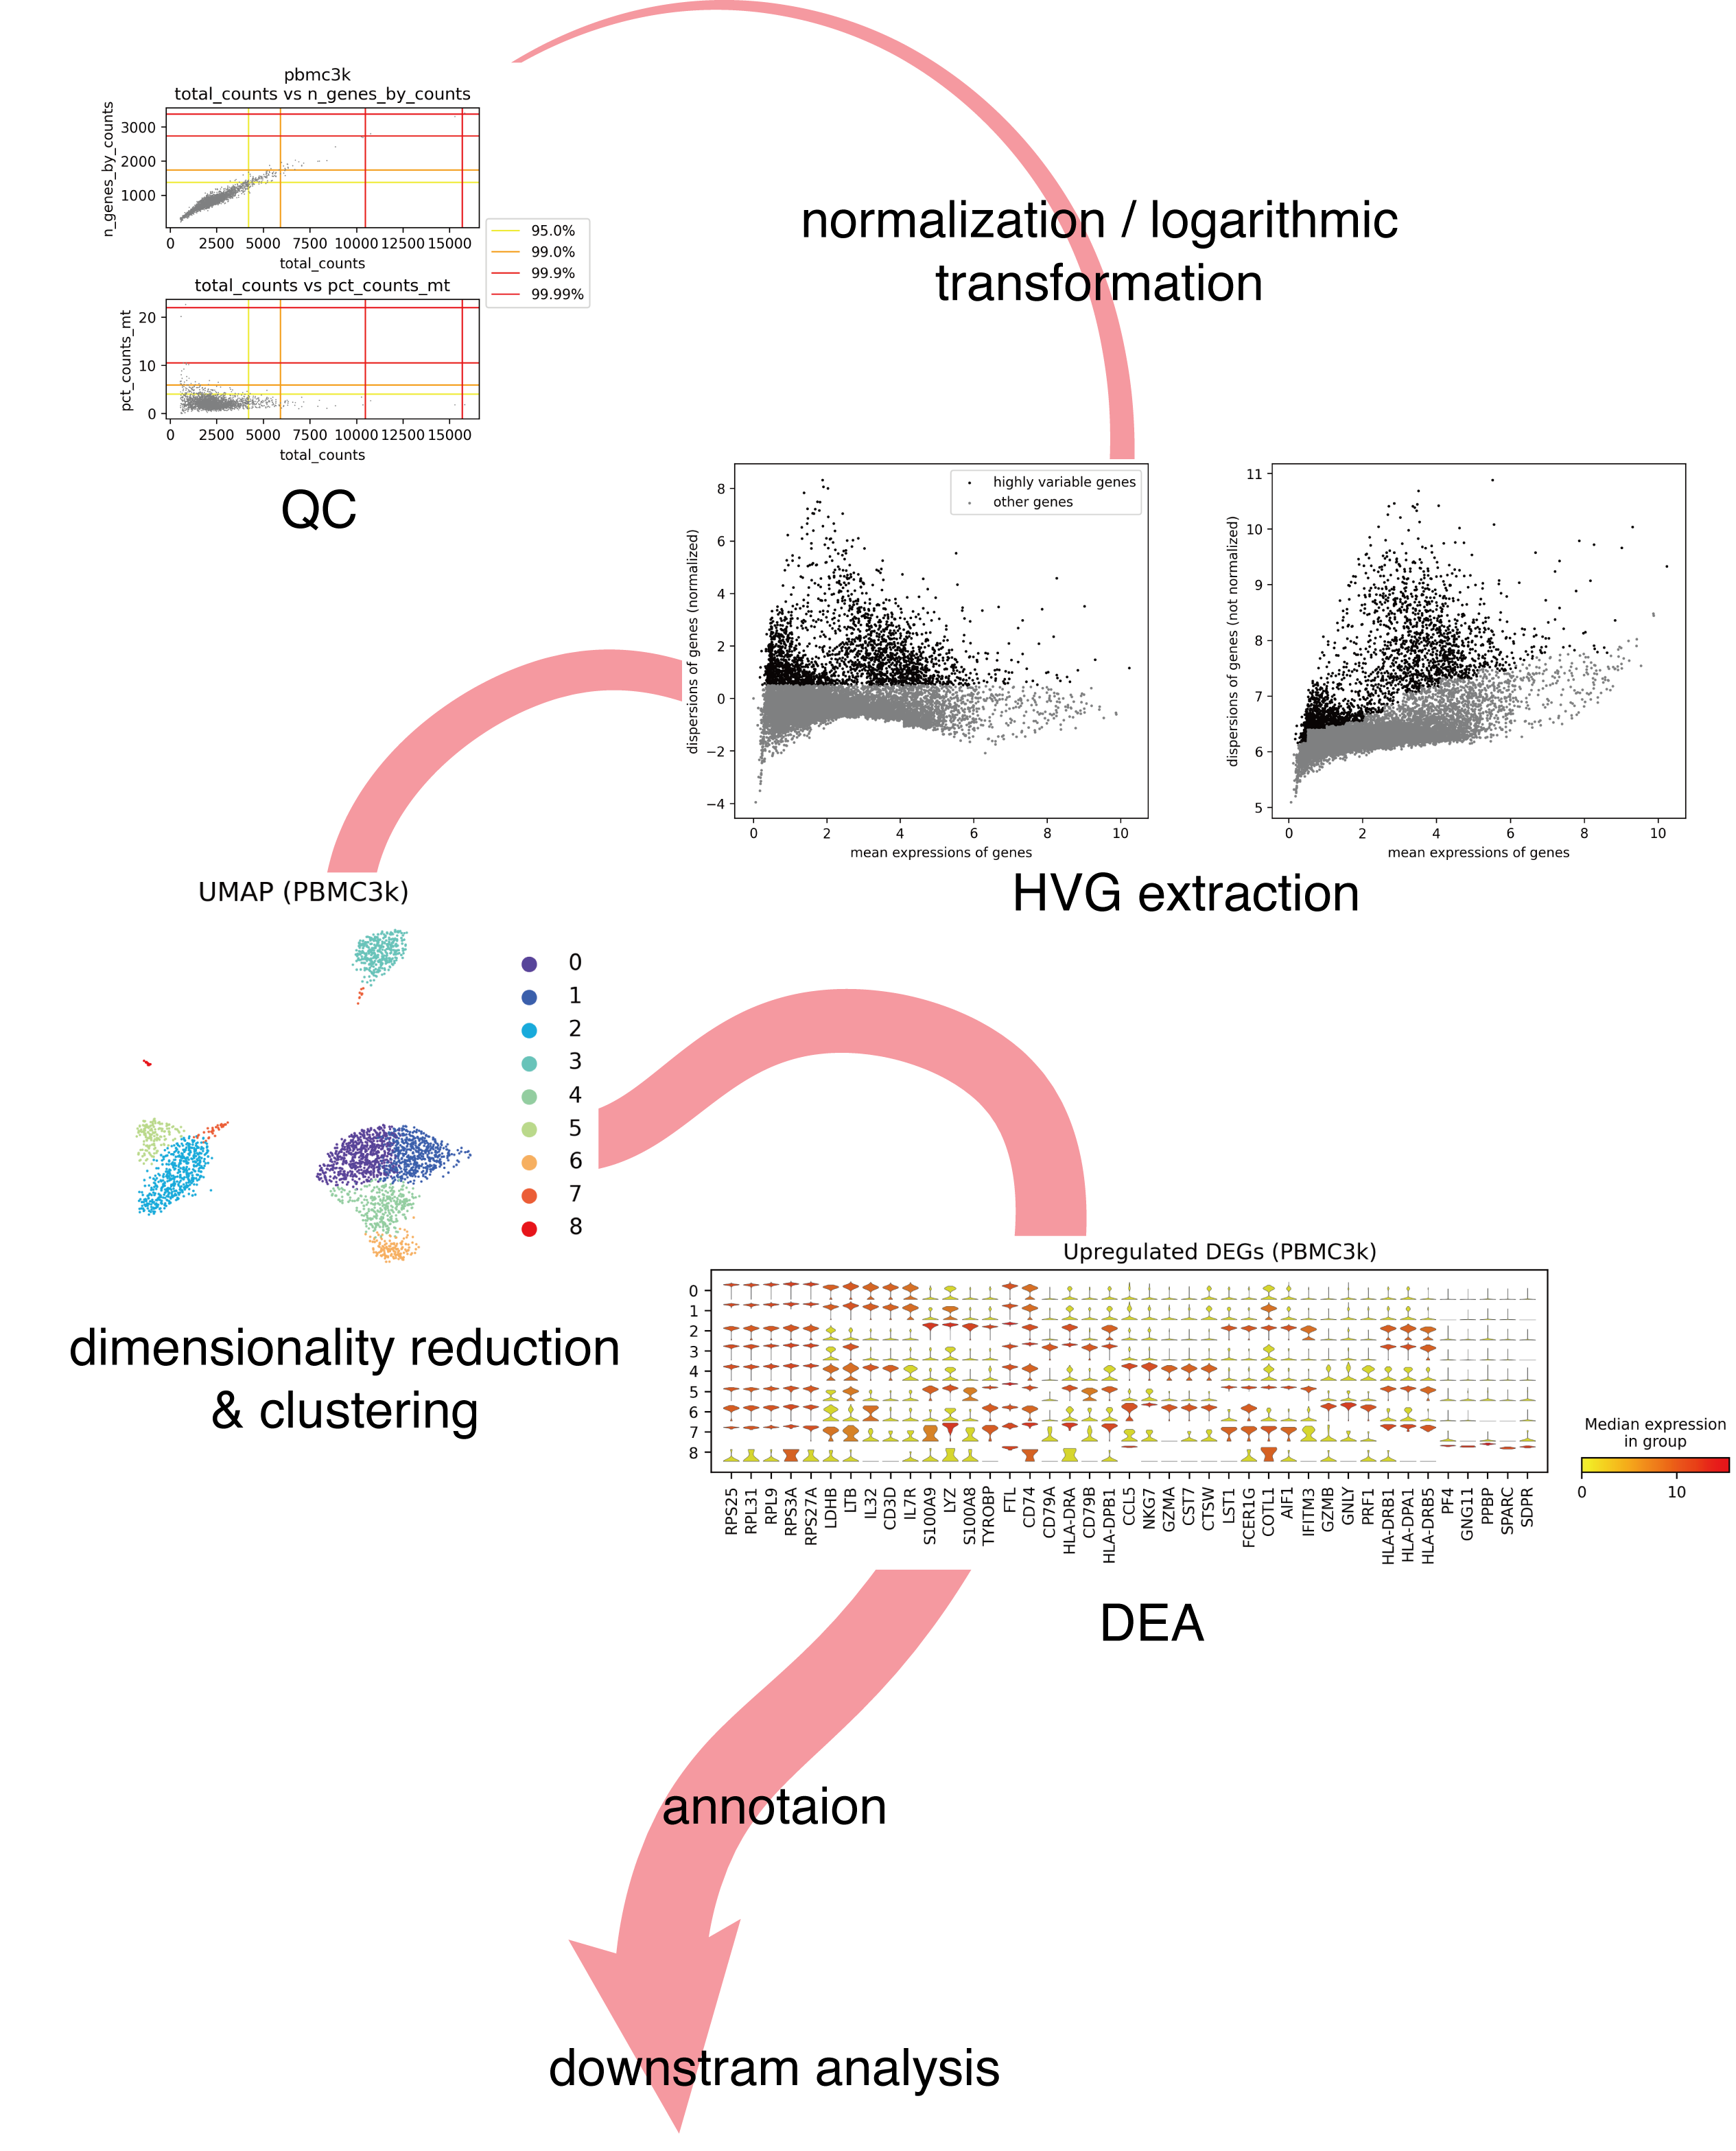
\includegraphics[scale=0.6]{./figs/exported/figure_s1.png}
  \caption{Gene expression patterns of clusters in PBMC3k}
  \legend{
    \textbf{A}: Violin plot of DEGs of the clusters (top 5 for each). 
    \textbf{B}: GRNs of the clusters. GRNs in a row share the same set of genes
    (DEGs of the subjective clusters) for the nodes
  }
  \label{fig_s1}
\end{figure}

\end{document}
